\chapter{System Design and Methodology}
\label{Chapter4}

This chapter describes the framework that was built for this thesis and the method used to evaluate it. Every statement about the framework in this chapter describes its code as it was used for the experiments. Section~\ref{sec:ch4-overview} gives the overall design. Sections~\ref{sec:ch4-stage0} to \ref{sec:ch4-stage4} describe the five stages. Section~\ref{sec:ch4-protocol} states the comparison protocol, Section~\ref{sec:ch4-search} describes the constrained search, and Section~\ref{sec:ch4-setup} gives the experimental setup.

\section{Overview of the Framework}
\label{sec:ch4-overview}

The framework is organised as five stages, shown in Figure~\ref{fig:ch4-overview}. Stage~0 measures how sensitive each decoder layer of the model is and turns the measurements into per-layer plans. Stages~1, 2 and 3 compress the model by following those plans: Stage~1 quantizes the weights and the activations, Stage~2 prunes weights, and Stage~3 compresses the KV cache. Stage~4 evaluates the resulting model in the inference engines. A search sits on top of the stages: it proposes which technique each stage should use and which settings Stage~0 should plan with, receives the Stage~4 measurements, and proposes the next configuration.

\begin{figure}[htbp]
\centering
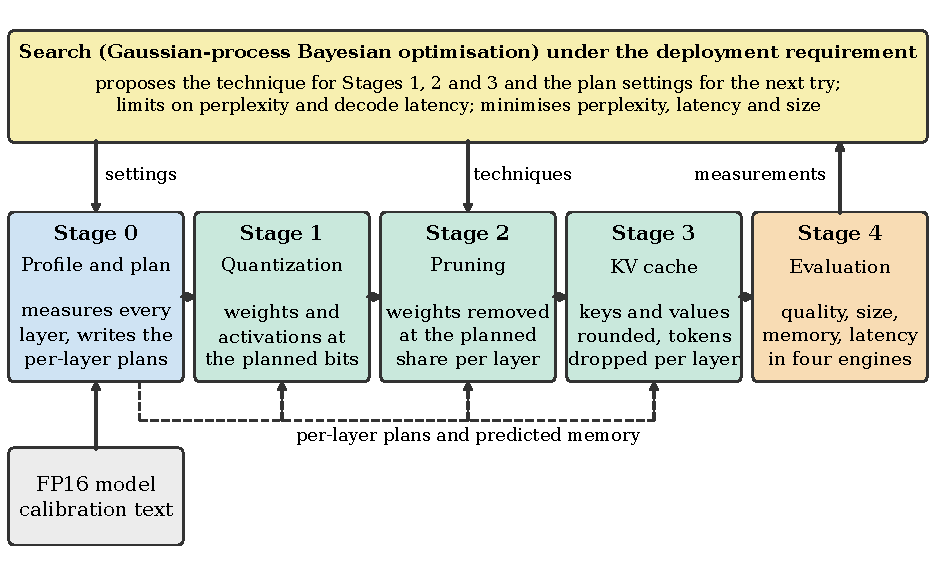
\includegraphics[width=\textwidth]{Figures/ch4-framework-overview.pdf}
\caption{The framework. Stage~0 measures the model and writes per-layer plans; Stages~1 to 3 compress the model following the plans; Stage~4 evaluates the result. The search proposes the techniques and the plan settings and receives the measurements.}
\label{fig:ch4-overview}
\end{figure}

The design separates two questions. Where to compress, that is, which layers keep more bits, which layers are pruned and how much of the cache each layer keeps, is decided once by Stage~0 and written into the plans. How to compress, that is, which published technique does the rounding or the pruning, is decided in Stages~1 to 3. Because of this separation, every technique can be run twice with the same code: once on a uniform plan that treats every layer the same, called \emph{Standard} in this thesis, and once on the Stage~0 plan, called \emph{Our method}. The only difference between the two runs is the plan.

The stages can be combined in two ways, listed in Table~\ref{tab:ch4-paths}. In the single-stage paths, one of Stages~1 to 3 is applied to a fresh copy of the FP16 model, so that the effect of each stage can be studied on its own. In the sequential path, Stages~1, 2 and 3 are applied one after another to the same model, and only the final model is evaluated.

\begin{table}[htbp]
\centering
\small
\caption{The paths through the framework that are evaluated in this thesis.}
\label{tab:ch4-paths}
\renewcommand{\arraystretch}{1.2}
\begin{tabularx}{\textwidth}{lX}
\hline
\textbf{Path} & \textbf{What is built and measured} \\
\hline
0 $\rightarrow$ 1 $\rightarrow$ 4 & Each quantization technique on the FP16 model, as Standard and as Our method. \\
0 $\rightarrow$ 2 $\rightarrow$ 4 & Each pruning technique on the FP16 model at each pruning level, as Standard and as Our method. \\
0 $\rightarrow$ 3 $\rightarrow$ 4 & Each KV-cache technique on the FP16 model, as Standard and as Our method. \\
0 $\rightarrow$ 1 $\rightarrow$ 2 $\rightarrow$ 3 $\rightarrow$ 4 & One model that is quantized, then pruned, then given a KV-cache technique. This is the path that the search uses. \\
\hline
\end{tabularx}
\end{table}

\section{Stage 0: Sensitivity Profiling and Planning}
\label{sec:ch4-stage0}

Stage~0 takes the FP16 model and a sample of calibration text and produces four things: a sensitivity score for each decoder layer, a weight plan, an activation plan and a KV-cache plan, each with a prediction of the memory it will need. The measurements depend only on the model and the calibration data, so they are stored in a cache on disk and reused by every later run that has the same model, data and seed.

\subsection{Calibration and Evaluation Data}
\label{sec:ch4-data}

The calibration data are 64 windows of 512 tokens, drawn at random positions from the shuffled documents of the training split of WikiText-2 with a fixed seed. The evaluation data are the test split of WikiText-2, joined into one text and cut into windows of 512 tokens that do not overlap. The first half of the windows is the validation set and the second half is the held-out set. Every decision in the framework, including every decision of the search, uses the validation set only. The held-out perplexity is measured and reported next to it, but it is never used to choose anything.

\subsection{Sensitivity Score}
\label{sec:ch4-score}

The default sensitivity score is a direct measurement. For each decoder layer $l$, the layer is bypassed, so that its input is passed straight to the next layer, and the perplexity on the calibration text is measured again. The raw score is the rise in perplexity:
\begin{equation}
  r_l = \mathrm{PPL}_{\mathrm{calib}}(\text{model with layer } l \text{ bypassed}) - \mathrm{PPL}_{\mathrm{calib}}(\text{model}).
  \label{eq:ch4-score}
\end{equation}
This needs one pass over the calibration text for the unchanged model and one pass for each layer. The raw scores are then rank-normalised: the layers are sorted by $r_l$ and layer $l$ receives $s_l = \mathrm{rank}(r_l) / (n - 1)$, where $n$ is the number of layers and tied layers share the average rank. The most sensitive layer therefore has $s_l = 1$ and the most robust has $s_l = 0$. Six other scores are implemented and can be selected in place of the default: the perplexity rise when only layer $l$ is rounded, gradient times weight, Fisher, Taylor, Hessian diagonal and movement scores. The experiments in this thesis use the default score.

\subsection{Weight Plan}
\label{sec:ch4-weightplan}

The weight plan gives each decoder layer a bit width $b_l$ and a pruning ratio $p_l$. It is made from the normalised scores with one threshold $\tau$ and one pruning ratio $\rho$:
\begin{equation}
  (b_l,\; p_l) = \left\{
  \begin{array}{ll}
    (8,\; 0) & \text{if } s_l \geq \tau \quad \text{(protected layer)} \\
    (4,\; \rho) & \text{if } s_l < \tau \quad \text{(compressed layer)}
  \end{array}
  \right.
  \label{eq:ch4-plan}
\end{equation}
A second rule, the guard, is applied on top: the five layers with the largest raw score $r_l$ are never pruned, whatever the threshold is. The default values are $\tau = 0.5$ and $\rho = 0.3$; both are settings that the search can change (Section~\ref{sec:ch4-search}). Only the linear weight matrices inside the decoder layers are compressed. The embeddings, the normalisation layers and the output head stay in 16-bit floating point in every plan.

From this rule Stage~0 writes separate plan files for the later stages: a quantization plan with the bit widths only, used by Stage~1, and a pruning plan with the pruning ratios only, used by Stage~2. For the pruning experiments it also writes one pruning plan for each pruning level from 30 to 90 percent, and for each level a second plan that removes exactly as many weights in total as the Standard plan does but places them by sensitivity. In that plan, layer $l$ is pruned at $\min(1,\; c\,(1 - s_l + 1/(n-1)))$, guarded layers are not pruned, and the constant $c$ is chosen so that the total number of removed weights equals the level times the number of decoder weights. Since the bits and the number of weights kept are the same as in the Standard plan, any difference in quality between the two comes only from where the pruning is placed.

\subsection{Activation Plan}
\label{sec:ch4-actplan}

The activation plan gives each layer a bit width for its activations. Stage~0 measures it in the same direct way as the weights: for each layer and for each candidate bit width (4 and 8 bits), the inputs of every linear module of that layer are rounded to that bit width while all other layers are left unchanged, and the rise in calibration perplexity is recorded. The plan then spends an average of 6 bits per layer. Every layer starts at 4 bits, and the layers are raised to 8 bits one at a time, taking first the layer for which the upgrade removes the most measured damage per extra bit, until the budget is used. The Standard activation plan gives every layer 8 bits.

\subsection{KV-cache Plan}
\label{sec:ch4-kvplan}

The KV-cache plan gives each layer a bit width for its cached keys, a bit width for its cached values, and the share of past tokens that the layer keeps. For the bit widths, Stage~0 rounds the keys of one layer (per channel, before the rotary position encoding is applied) or the values of one layer (per token) to 2, 4 and 8 bits in turn and records the rise in calibration perplexity. The bits are then allocated with the same greedy rule as in the activation plan, under an average of 4 bits per cached number, which is the size of the Standard plan (every key and value at 4 bits). For the share of tokens, Stage~0 records, for each layer and for keep ratios of 10, 20, 30, 50 and 75 percent, how much of the layer's attention falls on the most-attended tokens. The layer is given the smallest keep ratio that still covers 95 percent of its attention. The memory of a cache plan is predicted for a context of 2{,}048 tokens and a batch of one.

\subsection{Predicted Memory}
\label{sec:ch4-cost}

For every weight plan Stage~0 predicts the memory of the compressed weights without building a model. With $N_l$ the number of weights of layer $l$, $g$ the quantization group size and $N_{\mathrm{other}}$ the number of parameters outside the decoder weight matrices, the predicted number of bits is
\begin{equation}
  B = \sum_{l} \left[ N_l (1 - p_l)\, b_l \;+\; \frac{N_l (1 - p_l)}{g} \cdot 32 \;+\; m_l N_l \right] \;+\; 16\, N_{\mathrm{other}},
  \label{eq:ch4-cost}
\end{equation}
where the second term counts one 32-bit scale and zero-point pair per group of kept weights, and $m_l = 1$ for a layer that is partly pruned and $0$ otherwise, which counts a one-bit mask that records which weights are kept. A layer that stays at 16 bits has no scale term. For techniques that store additional data of their own, such as codebooks or outliers, that data replaces the scale term. The search uses this prediction to reject a configuration that is over a size limit before spending time on building it. The prediction describes the plan, not an exported file; the real file sizes are measured in Stage~4.

Table~\ref{tab:ch4-stage0-settings} lists the Stage~0 settings.

\begin{table}[htbp]
\centering
\small
\caption{Stage~0 settings used in the experiments.}
\label{tab:ch4-stage0-settings}
\renewcommand{\arraystretch}{1.15}
\begin{tabularx}{\textwidth}{Xl}
\hline
\textbf{Setting} & \textbf{Value} \\
\hline
Model & TinyLlama-1.1B-Chat-v1.0 \cite{zhang2024tinyllama} \\
Calibration data & WikiText-2, 64 windows of 512 tokens \\
Sensitivity score; normalisation & perplexity rise when the layer is bypassed; rank \\
Sensitivity threshold $\tau$ (default) & 0.5 \\
Bits of protected / compressed layers & 8 / 4 \\
Pruning ratio $\rho$ of compressed layers (default) & 0.3 \\
Guard: layers never pruned & 5 with the largest raw score \\
Quantization group size (default) & 128 weights \\
Standard weight plan & 4 bits in every layer \\
Activation bit options; average budget; Standard & 4 and 8; 6 bits; 8 bits in every layer \\
KV bit options; average budget; Standard & 2, 4 and 8; 4 bits; 4 bits in every layer \\
KV keep ratios; attention coverage & 0.1, 0.2, 0.3, 0.5, 0.75; 0.95 \\
Standard share of tokens kept by eviction methods & 0.2 \\
Pruning levels & 0.3 to 0.9 in steps of 0.1 \\
Seed & 0 \\
\hline
\end{tabularx}
\end{table}

\section{Stage 1: Quantization}
\label{sec:ch4-stage1}

Stage~1 rounds the weights and the activations of the model to the bit widths in the plan and removes nothing. Its techniques fall into three kinds, listed in Table~\ref{tab:ch4-stage1}. Weight techniques round the weight matrices. Activation techniques round or transform the inputs of the linear modules. A combined technique, written as a weight technique with an activation technique, applies both to one model: the activation technique first rewrites the model, the weight technique then rounds the weights, and the activations are rounded while the model is measured. Each layer of a combined model therefore has its own pair of weight bits and activation bits.

The basic rounding operation is the uniform affine quantizer of Equation~\ref{eq:ch2-quant}, applied per group of $g$ consecutive weights with the scale taken from the minimum and maximum of the group and an integer zero-point. Round-to-nearest applies this operation directly. GPTQ rounds a weight matrix column by column and compensates the error of each column in the columns that are not yet rounded, using second-order information from the calibration inputs of the layer \cite{frantar2023gptq}; in the framework the layers are processed in order, and each layer is calibrated on inputs that have passed through the layers already rounded. AWQ scales the weight channels according to the size of their activations before rounding \cite{lin2024awq}. The other techniques are published methods that were re-implemented in simplified form inside the framework so that they can follow a per-layer plan, as stated in Section~\ref{sec:ch1-scope}; the simplifications of each technique are recorded with its results.

\begin{table}[htbp]
\centering
\small
\caption{Stage~1 techniques. Each weight technique can be combined with round-to-nearest activations or with SmoothQuant.}
\label{tab:ch4-stage1}
\renewcommand{\arraystretch}{1.2}
\begin{tabularx}{\textwidth}{lX}
\hline
\textbf{Kind} & \textbf{Techniques} \\
\hline
Weights & Round-to-nearest; GPTQ \cite{frantar2023gptq}; AWQ \cite{lin2024awq}; OmniQuant \cite{shao2024omniquant} (learnable weight clipping only); SqueezeLLM \cite{kim2024squeezellm}; SpQR \cite{dettmers2024spqr}; EfficientQAT \cite{chen2025efficientqat} (block-wise step only); QuIP \cite{chee2023quip}; QuIP\# \cite{tseng2024quipsharp}; PB-LLM \cite{shang2023pbllm}; BiLLM \cite{huang2024billm} (Standard only); the 4-bit and 8-bit storage of the bitsandbytes library \\
Activations & Round-to-nearest activations; SmoothQuant \cite{xiao2023smoothquant}; QuaRot \cite{ashkboos2024quarot}; SpinQuant \cite{liu2025spinquant}; RPTQ \cite{yuan2023rptq} (Standard only) \\
\hline
\end{tabularx}
\end{table}

Two remarks apply to this table. First, EfficientQAT is included only with its block-wise step, which trains the quantization parameters of one block at a time on the calibration data; its end-to-end training step is not run. Second, in the Standard run a weight technique uses 4 bits in every layer, and a combined technique uses 4-bit weights and 8-bit activations in every layer; in the Our method run the same technique uses the Stage~0 quantization plan and, for a combined technique, the Stage~0 activation plan.

In Stages~1 to 3 the compression is simulated in Hugging Face Transformers: the rounded values are written back into 16-bit floating-point tensors. The quality measured on this model is the quality of the rounding itself. Its size and speed are not real, which is why the model is exported to the inference engines in Stage~4.

\section{Stage 2: Pruning}
\label{sec:ch4-stage2}

Stage~2 removes weights and rounds nothing. It has three techniques.

\begin{itemize}
  \item \textbf{Unstructured pruning} uses the Wanda criterion: within each output row of a weight matrix, the weights with the smallest product of weight magnitude and input activation norm are set to zero, with no weight update \cite{sun2024wanda}.
  \item \textbf{Structured pruning} removes whole inner channels of the feed-forward network of a layer, that is, a row of each input matrix and the matching column of the output matrix. Channels are removed in increasing order of the product of the channel's activation norm and the norm of its output column, until the planned share of the layer's weights is removed. At most 75 percent of a layer is removed, and attention heads are never removed.
  \item \textbf{Low-rank factorisation} replaces each weight matrix by a product of two smaller matrices obtained from an activation-aware singular value decomposition, following the ASVD idea \cite{yuan2025asvd}. The rank is chosen so that the layer keeps the planned share of its numbers. This technique cannot follow Stage~1 and is therefore used only in the path 0 $\rightarrow$ 2 $\rightarrow$ 4.
\end{itemize}

Each technique is run at every pruning level from 30 to 90 percent. In the Standard run the level is removed from every layer. In the Our method run the level is removed from the layers that Stage~0 found robust, and nothing is removed from the protected and guarded layers. A third run uses the same-size plan of Section~\ref{sec:ch4-weightplan}, which removes the same total as the Standard run. In addition, Stage~0 runs a pruning-levels test in which each technique prunes the FP16 model at each level on three sets of layers (all layers, all layers except the guarded ones, and the guarded layers only), which shows how much of the damage of pruning comes from the guarded layers.

Removed weights are stored as zeros. As stated in Section~\ref{sec:ch1-scope}, the pruning experiments therefore measure quality only.

\section{Stage 3: KV-cache Compression}
\label{sec:ch4-stage3}

Stage~3 compresses the KV cache and leaves the weights as they are. Its techniques, listed in Table~\ref{tab:ch4-stage3}, are of two kinds: rounding techniques store the cached keys and values in fewer bits, and eviction techniques keep only part of the past tokens. All of them are implemented inside the attention computation of the Hugging Face model: keys and values are rounded in place, and evicted tokens are masked out of the attention. The cache memory reported for a technique is the prediction of its plan, for a context of 2{,}048 tokens and a batch of one.

\begin{table}[htbp]
\centering
\small
\caption{Stage~3 techniques as implemented in the framework.}
\label{tab:ch4-stage3}
\renewcommand{\arraystretch}{1.2}
\begin{tabularx}{\textwidth}{lX}
\hline
\textbf{Technique} & \textbf{Implementation in the framework} \\
\hline
Round-to-nearest KV & Keys rounded per channel before the position encoding, values per token, with the same rounding as the Stage~0 measurement. \\
QuaRot KV \cite{ashkboos2024quarot} & Keys and values rotated by a Hadamard matrix and then rounded. \\
KVQuant \cite{hooper2024kvquant} & Keys per channel before the position encoding and values per token, with non-uniform levels found by k-means and one percent of outliers left unrounded. The levels are not weighted by sensitivity as in the paper. \\
H2O \cite{zhang2023h2o} & A cache of fixed size per layer, half for the most recent tokens and half for the heavy-hitter tokens. \\
SnapKV \cite{li2024snapkv} & An observation window of the latest tokens and the earlier tokens that the window attends to most, in a cache of the same fixed size as H2O. \\
InfiniGen \cite{lee2024infinigen} & The tokens to keep are predicted from 30 percent of the channels, in a cache of the same fixed size as H2O. The offloading of the full cache to CPU memory described in the paper is not run. \\
\hline
\end{tabularx}
\end{table}

In the Standard run a rounding technique stores every key and value at 4 bits and keeps every token, and an eviction technique keeps 20 percent of the past tokens at full precision. In the Our method run each technique follows the Stage~0 KV-cache plan: the planned key bits, value bits and share of tokens for each layer.

\section{Stage 4: Evaluation}
\label{sec:ch4-stage4}

Stage~4 measures a model. It always measures the simulated model in Hugging Face Transformers \cite{wolf2020transformers}, and it exports the model to llama.cpp \cite{ggml2025llamacpp} and vLLM \cite{kwon2023vllm} to measure real file size, memory and speed. An export to TensorRT-LLM \cite{nvidia2025tensorrtllm} is also implemented, but no TensorRT-LLM measurement is reported in this thesis.

\subsection{Measurements in Hugging Face Transformers}
\label{sec:ch4-hf}

Perplexity is computed with Equation~\ref{eq:ch2-ppl} over the validation windows and, separately, over the held-out windows. Latency is measured at batch size one with a random prompt of 128 tokens: the prefill time is the time to process the prompt, and the decode latency is the time per token over 64 greedy decoding steps with a pre-allocated KV cache. On a GPU the prefill and one decoding step are each captured once as a CUDA graph and replayed, so that the measured time is the work of the GPU and not the overhead of Python; when a technique prevents the capture, the same loop is run without it and the result records which mode ran. Each measurement is preceded by 3 warm-up runs and repeated 10 times, and the mean and the standard deviation are reported. The model size and the peak GPU memory are also recorded. Zero-shot accuracy on ARC-Easy, PIQA, HellaSwag and WinoGrande (Section~\ref{sec:ch2-metrics}) is measured with the lm-evaluation-harness library on the model as compressed, so that the tasks see exactly what a technique changed.

\subsection{Export to the Inference Engines}
\label{sec:ch4-export}

Table~\ref{tab:ch4-engines} summarises how a model reaches each engine. In every case the per-layer bit widths of the plan are kept in the exported file, and the embeddings and the output head stay in 16-bit floating point.

\begin{table}[htbp]
\centering
\small
\caption{How a compressed model is exported to and measured in each inference engine.}
\label{tab:ch4-engines}
\renewcommand{\arraystretch}{1.2}
\begin{tabularx}{\textwidth}{lX}
\hline
\textbf{Engine} & \textbf{Export and measurement} \\
\hline
llama.cpp & The model is converted to GGUF \cite{ggml2025gguf} and quantized with llama.cpp's own quantization types, each decoder layer at its planned bit width. Speed is measured with the llama-bench program and perplexity with the llama-perplexity program, which scores the second half of each window. \\
vLLM, weights only & The model is saved as a GPTQ-format checkpoint with per-layer bit widths of 2, 3, 4 or 8 bits. The weights are re-rounded onto symmetric per-group grids, because vLLM loads only symmetric grids in this format. \\
vLLM, weights and activations & The model is saved as a compressed-tensors checkpoint in which each decoder layer has its own weight bits and activation bits; vLLM rounds the activations while the model runs. \\
TensorRT-LLM (implemented, not measured in this thesis) & The same GPTQ-format checkpoint is built into a TensorRT engine, with one bit width or with a per-layer mixed-precision configuration. \\
\hline
\end{tabularx}
\end{table}

vLLM and TensorRT-LLM run in Python environments of their own, separate from the framework, and are started by the framework as worker processes. In both, the latency is measured with the same prompt length, number of decoded tokens, warm-up runs and repeats as in Hugging Face: the prefill time is the time of a request that generates one token after the 128-token prompt, and the decode latency is the time of a request that generates 64 tokens minus the prefill time, divided by 63. Prefix caching is switched off so that every prefill is a real one.

Three properties of the exports matter for reading the results in Chapter~5. First, each engine re-rounds the weights onto its own grid, so a perplexity measured in an engine is comparable with other perplexities measured in the same engine, and not with the Hugging Face perplexity. Second, in vLLM the weight-only models and the models with rounded activations run on different kernels: in the experiments of this thesis a weight-only model decodes in about 2~ms per token, while a model with rounded activations decodes in about 35 to 42~ms per token. Decode latencies of the two kinds are therefore comparable only within each kind. Third, some models cannot be exported: models rewritten by QuaRot or SpinQuant need a rotation at run time that the export formats do not carry, and the KV-cache techniques of Stage~3 exist only in the Hugging Face model. Models of the path 0 $\rightarrow$ 3 $\rightarrow$ 4 are therefore measured in Hugging Face only.

\section{Comparison Protocol}
\label{sec:ch4-protocol}

Every experiment in the single-stage paths reports three kinds of row for each technique:

\begin{itemize}
  \item \textbf{FP16}: the uncompressed model.
  \item \textbf{Standard}: the technique on the uniform plan (for example 4-bit weights in every layer, or 4-bit weights and 8-bit activations in every layer).
  \item \textbf{Our method}: the same technique, with the same code, on the Stage~0 plan.
\end{itemize}

The three rows are produced under identical conditions: the same calibration windows, the same seed, the same evaluation windows, the same GPU and the same engine versions. Every row starts from a fresh copy of the FP16 model, so that no row is affected by an earlier one. Results that are expensive to compute, such as the FP16 measurements and the sensitivity measurements, are stored in a cache whose key contains every setting that determines them, so that a result is reused only when all of those settings are equal. A row that fails is kept in the results with its error message; it is not removed.

\section{Constrained Multi-objective Search}
\label{sec:ch4-search}

The search answers the question of which combination of techniques and settings to use for a given deployment requirement. Figure~\ref{fig:ch4-search} shows one search run.

\begin{figure}[htbp]
\centering
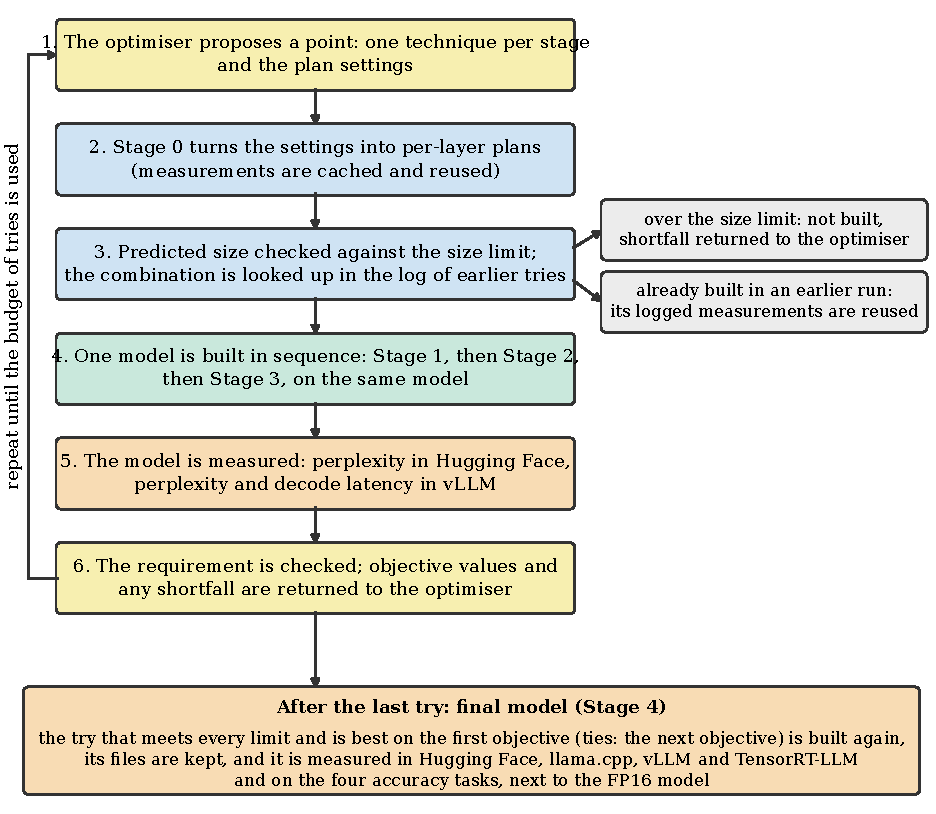
\includegraphics[width=0.95\textwidth]{Figures/ch4-search-loop.pdf}
\caption{One run of the search. Each try builds one model through Stages~1, 2 and 3 in sequence and measures it. After the last try the final model is evaluated in the engines and on the accuracy tasks.}
\label{fig:ch4-search}
\end{figure}

\subsection{Deployment Requirement and Objectives}
\label{sec:ch4-requirement}

A deployment requirement is a set of upper limits. The framework supports limits on validation perplexity, on decode latency, on weight memory and on KV-cache memory. The requirement used in this thesis has two limits: a validation perplexity of at most 11.5 and a vLLM decode latency of at most 2.5~ms per token. The perplexity limit can be checked on the Hugging Face model or on the model as loaded in vLLM; Chapter~5 states which was used for each search. For a model that misses a limit, the framework records the shortfall, that is, by how much each limit was missed.

Within the limits the search minimises up to three objectives: validation perplexity, vLLM decode latency and predicted weight memory. The objectives of each search run are given with its results in Chapter~5. The held-out perplexity cannot be selected as an objective or as a limit.

\subsection{Search Space}
\label{sec:ch4-space}

A point of the search space consists of one technique for each of Stages~1, 2 and 3 and of the numeric settings in Table~\ref{tab:ch4-space}. The Stage~1 choices are the weight techniques round-to-nearest, GPTQ, AWQ, OmniQuant, SqueezeLLM, SpQR, EfficientQAT, QuIP, QuIP\#, PB-LLM and bitsandbytes, each combined with round-to-nearest activations or with SmoothQuant, and in addition round-to-nearest, GPTQ, AWQ, OmniQuant and EfficientQAT as weight-only techniques. The Stage~2 choices are unstructured and structured pruning. The Stage~3 choices are the six techniques of Table~\ref{tab:ch4-stage3}.

\begin{table}[htbp]
\centering
\small
\caption{Numeric settings of the search space.}
\label{tab:ch4-space}
\renewcommand{\arraystretch}{1.2}
\begin{tabularx}{\textwidth}{Xll}
\hline
\textbf{Setting} & \textbf{Full range} & \textbf{Range set for the search} \\
\hline
Sensitivity threshold $\tau$ & 0.1 to 0.9 & 0.8 to 0.9 \\
Pruning ratio $\rho$ of compressed layers & 0.0 to 0.6 & 0.0 to 0.3 \\
Calibration dataset & WikiText-2, C4, Pile (10k sample) & as full range \\
Number of calibration windows & 16, 32, 64, 128 & as full range \\
Quantization group size & 32, 64, 128, per channel & as full range \\
SmoothQuant migration strength & 0 to 1 & as full range \\
\hline
\end{tabularx}
\end{table}

\subsection{Evaluating One Point}
\label{sec:ch4-point}

For each point, Stage~0 makes the plans for the point's settings. The predicted weight memory of the plan (Equation~\ref{eq:ch4-cost}) is checked first; a point that is over a memory limit is not built. Otherwise one model is built in sequence: the Stage~1 technique quantizes the FP16 model following the quantization and activation plans, the Stage~2 technique prunes that model following the pruning plan, and the Stage~3 technique is applied to the result following the KV-cache plan. Only the Our method side is built. The model is then measured in Hugging Face, and also in vLLM when an objective or a limit is a vLLM measurement. llama.cpp and TensorRT-LLM are not run during the tries.

Two mechanisms prevent the same model from being built twice. Within a run, a model is built once per plan: two thresholds that fall between the same two layers give the same plan and therefore share one model. Across runs, every combination that has been tried is written to a log file that is kept with the cache. When a later run proposes a combination that is already in the log, the logged measurements are used, the requirement is checked again, and nothing is built. A search can therefore be extended with more tries without repeating earlier ones.

\subsection{Optimiser}
\label{sec:ch4-optimiser}

The optimiser is multi-objective Bayesian optimisation (Section~\ref{sec:ch2-moo}), for which the framework uses the Gaussian-process sampler of the Optuna library. All objectives are minimised, and the requirement is passed to the sampler as a constraint whose value is the sum of the shortfalls of the point, which is zero for a point that meets every limit. A point that was not built because its plan is over a limit, or that failed while being built or measured, is reported to the sampler with the worst objective values seen so far and a positive constraint value, so that the sampler learns to avoid that region. The run ends when the budget of tries is used. A point that is not built because its plan is over a limit does not use up the budget.

Two other optimisers are implemented in the framework: successive halving \cite{bischl2021hpo}, which evaluates many points on a fraction of the evaluation windows and keeps the best third at each of three rounds, and NSGA-III through the pymoo library \cite{blank2020pymoo}. The search results in Chapter~5 come from the Bayesian optimiser.

\subsection{Final Model}
\label{sec:ch4-final}

After the last try, the final model is selected among all tries, of this run and of earlier runs in the log, that were measured on the full validation set and meet every limit. The selected try is the one with the lowest value of the first objective; ties are broken by the second objective and then by the third. This model is built again and its exported files are kept. It is then evaluated in the engines that are installed on the machine of the run (Hugging Face and vLLM for the searches of Chapter~5) and on the four accuracy tasks. The FP16 model is evaluated on the same tasks in the same run, so that the two accuracies are measured under the same conditions. When no try meets every limit, no final model is selected, and the report lists the tries with their shortfalls.

\section{Experimental Setup}
\label{sec:ch4-setup}

All experiments use TinyLlama-1.1B-Chat-v1.0 (Section~\ref{sec:ch2-tinyllama}) and the settings of Table~\ref{tab:ch4-stage0-settings}. Table~\ref{tab:ch4-setup} lists the hardware and software. The seed fixes the random number generators of Python, NumPy and PyTorch, and the deterministic mode of PyTorch is switched on where a deterministic implementation exists. Each configuration is run with this one seed (Section~\ref{sec:ch1-scope}).

\begin{table}[htbp]
\centering
\small
\caption{Hardware and software of the experiments.}
\label{tab:ch4-setup}
\renewcommand{\arraystretch}{1.2}
\begin{tabularx}{\textwidth}{lX}
\hline
\textbf{Item} & \textbf{Value} \\
\hline
GPUs & NVIDIA A100 80~GB on Google Colab; NVIDIA RTX~5070~Ti 16~GB in a desktop PC \\
Framework & Python 3.10 or later, PyTorch 2.1 or later, Transformers 4.56 or later \\
Search & Optuna 5 or later (Gaussian-process sampler); pymoo 0.6 or later (NSGA-III option) \\
Accuracy tasks & lm-evaluation-harness 0.4 or later \\
vLLM & version 0.31.0, in its own Python environment (Linux only) \\
TensorRT-LLM & version 1.2, in its own Python environment (Linux only); not measured in this thesis \\
llama.cpp & release programs with CUDA support \\
\hline
\end{tabularx}
\end{table}

Because vLLM runs on Linux only, every measurement that involves it, including all search runs, was made on the A100. Every run writes its configuration, a log, a table of all rows and a report to its own folder, and the tables and figures of Chapter~5 are taken from these files.

\section{Summary}
\label{sec:ch4-summary}

The framework separates where to compress from how to compress. Stage~0 measures each decoder layer directly, by the rise in calibration perplexity, and writes per-layer plans for the weights, the activations, pruning and the KV cache together with a prediction of their memory. Stages~1 to 3 apply published techniques that follow those plans, and each technique is also run on a uniform plan so that Standard and Our method differ only in the plan. Stage~4 measures the models in Hugging Face Transformers and, after export, in llama.cpp and vLLM. A constrained Bayesian search chooses one technique per stage and the plan settings under limits on perplexity and decode latency, builds each candidate as one model through Stages~1 to 3 in sequence, never builds the same combination twice, and selects a final model for full evaluation. Chapter~5 reports the results obtained with this method.
